\documentclass[12pt,a4paper]{article}
\usepackage[utf8]{inputenc}
\usepackage{amsmath}
\usepackage{amsfonts}
\usepackage{amssymb}
\usepackage[english]{babel}
\usepackage{graphicx}
\usepackage{siunitx}
\usepackage{pdfpages}
\usepackage{listings}
\usepackage{titlesec}

\titleformat*{\section}{\LARGE\bfseries}
\titleformat*{\subsection}{\LARGE\bfseries}
\titleformat*{\subsubsection}{\Large\bfseries}

\titleformat{\paragraph}
{\normalfont\large\bfseries}{\theparagraph}{1em}{}
\titlespacing*{\paragraph}
{0pt}{3.25ex plus 1ex minus .2ex}{1.5ex plus .2ex}

\begin{document}
\begin{titlepage}

\centering \parindent=0pt
\newcommand{\HRule}{\rule{\textwidth}{1mm}}
\vspace*{\stretch{1}} \HRule\\[0.7cm]\Huge\bfseries
30010 - Programmeringsprojekt \\[0.7cm] % Kursusnummer og navn
Reflexball\\ % Titel
\HRule\\[2cm]  
\Large
Gruppe 3
\\
\large
Martin Boye Brunsgaard, s144012(1)	\\
Tore Gederaas Kanstad, s144021(2) \\
Peter Asbjørn Leer Bysted, s144045(3) \\
\begin{figure}[h]
\begin{center}
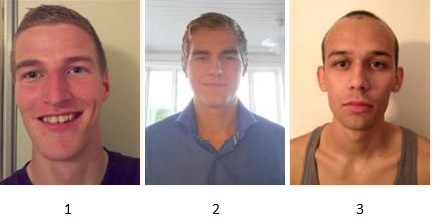
\includegraphics[scale=0.6]{img/faces.jpg}
\end{center}
\end{figure}

\vspace*{\stretch{1}} \normalsize

Alle medlemmer har været tilstede under øvelserne, og deltaget i udarbejdelse af journalerne. Ydermere har arbejdet været fordelt ligeligt over gruppemedlemerne, og løst i fællesskab. Rapporten er blevet udarbejdet og gennemlæst i kollektiv.
\vspace*{\stretch{1}}
\begin{flushleft}
Tecnical University of Denmark DTU\\ % Uddannelsesinstitusion
National Space Institute\\ 
30010 - Programming Project\\ % Kursusnummer og navn
25.06.2015 %Måned og år
\end{flushleft}
\end{titlepage}
\newpage
\renewcommand{\abstractname}{Abstract}
\begin{abstract}

This report covers the reflexbal game, which is a mandatory part of the B.Sc. EE course 30010 Programming Project.\\ The report documents the entire course of the exercises in which the digital logic behind a simple vending machine was designed using VHDL. The project was split into three sub-assignments: The first assignment was to drive a seven-segment display with hexadecimal numbers, the second was to display two different 2-digit decimal numbers simultaneously  and the last was to implement a CPU using a data path controlled by a FSM. The 3 assignements were combined into one circuit and implemented on a Basys2 Spartan FPGA board.
\end{abstract}
\newpage
\tableofcontents


\newpage
\section{Introduktion}
Målet med dette projekt er at designe og implementere et program. Programmet skal skrives i C og det skal implementeres på en Zilog Z8 encore microprocessor vha. ZDS II - Z8Encore! 4.9.3 værktøjer. Programmet skal dokumenteres vha. flowcharts, grafer og beskrivelser af de enkelte funktioner.

\begin{figure}[h]
\begin{center}
\includegraphics[scale=0.6]{img/reflexball.png}
\caption{Reflexball vist i PuTTY.}
\end{center}
\end{figure}

Programmet skal være et spil, Reflexball. Spilleren styrer en striker, som skal bruges til at reflektere en bold, således den kan bevæge sig rundt på banen. Hvis bolden rammer en af kanterne, skal bolden ligeledes også reflekteres. Hvis spilleren ikke rammer bolden ryger bolden ud af banen, og spilleren fratrækkes et liv. Såfremt spilleren ikke har flere liv tilbage, afsluttes spillet. Desuden indføres der nogle bokse i spillet, som spilleren skal ødelægge. Når spilleren har ødelagt alle disse bokse går spilleren videre til næste bane, eller vinder såfremt han er på sidste bane. Den grafiske flade bliver implementeret ved at skrive til en terminal. Ydermere får brugeren informationer fra LED'erne på boardet.


 
\section{Teori}

Vi vil i dette afsnit gennemgå den basale teori bag binære tal og slutteligt indføre læseren i de forskellige formater, deriblandt fixed-point format, og hvorfor det er interessant at bruge denne repræsentation  i vores projekt.
\subsection{Binære tal}
Et binært tal er et tal der kan udtrykkes i det binære talsystem/base-2, hvor grundtallet er 2. Da det er meget let at implementere i digital logik, er det et system der bruges internt i computere verden over. \\ 
Et binært tal består af bits, som svarer til et ciffer. Et bit kan have en af to tilstande: logisk højt eller logisk lavt. Dette medfører da hvis vi har \textit{n} bits har vi $2^n$ forskellige tilstande. Disse forskellige tilstande kan fortolkes på forskellige måder, og vi vil i de næste afsnit gennemgå nogle af de forskellige representationer.
\subsection{Unsigned repræsentation}
I det binære talsystem er grundtallet vanligvis 2(det kunne potentielt også være -2). Det betyder således at i en n-bit streng, vil  bittet yderst til højre være vægtet med  $2^0$, det næste med $2^1$ op til $2^n$ gående mod venstre. Tallet 5(base-10) kan da skrives som i ligning \ref{unsigned}. Ydermere tæller vi også fra højre mod venstre, og første bit står såldedes også på 0 plads. Dette bit kaldes oftest LSB(least significant bit), hvorimod det bit der står helt til venstre kaldes MSB(most significant bit).


\begin{equation}\label{unsigned}
5_{10} = 101_{2} = 1 \cdot 2^2+0 \cdot 2^1+1 \cdot 2^0
\end{equation}


Med de indførte definitioner har vi kun mulighed for at repræsentere positive heltal. Vi ønsker også at kunne skrive kommatal og negative tal.

\subsection{Fixed point kommatal}
Kommatal kan indføres på en simpel måde, ved blot at vægte i omvendt retning når man går mod højre, således at bittet til højre for kommaet har vægtningen $2^{-1}$, bittet 2 til højre for kommat vægtningen $2^{-2}$ osv. Hvis man har en n-bit streng med b tal til højre for kommaet, har man da muligheden for at skrive tal mellem 0 og $\frac{2^n-1}{2^b}$ \cite[s.~4]{Yates}

Tallet 13.625 kan f.eks skrives som

\begin{equation}
13.625_{10} = 1101.101_2 = 1 \cdot 2^3+1 \cdot 2^2+1 \cdot 2^0+1 \cdot 2^{-1}+1 \cdot 2^{-3}
\end{equation}

\subsection{Repræsentation af negative tal}
Hvis vi ønsker at repræsentere negative tal, gøres det oftest på 3 forskellige måder: 
Signed magnitude, 1's kompliment eller 2's kompliment. Vi vil her gennemgå signed magnitude og 2's komplement.
\subsubsection{Signed magnitude}
En af måderne at repræsentere fortegnet på bit-strengen, er ved at lade det mest signifikante bit(MSB: længst til venstre) bestemme fortegnet, hvor 0 indikerer et positivt tal og 1 indikerer et negativt tal.  F.eks. kan tallet -37 i signed magnitude repræsentation skrives således:
\begin{equation}
-37_{10} = 1100101_2 
\end{equation}
Signed magnitude repræsentation, har dog den ulempe, at man spilder et bit, f.eks. hvis man har en 4-bit streng gælder der at 1000 =  0000, så istedet for at have $2^4$ tilstande har man blot $2^4-1$. 
\subsubsection{2's komplement}
En anden måde at repræsentere negative tal, kan gøres vha. 2's komplement. 2's komplement findes ved at invertere et unsigned tal og derefter lægge 1 til. 2's komplement har to fordele: Der er kun et 0, og subtraktion kan gøres på samme måde som addition, så hvis vi ønsker at subtrahere 3 fra 5, skal vi blot finde 2's kompliment af 3 og lægge det til 5, som i \ref{2skomp}
\begin{equation}
\label{2skomp}
 5-3 = 5+(-3)
\end{equation}
Disse fordele gør 2's komplement et af de mest udbredte metoder til at repræsentere negative tal i digitale systemer.

\subsection{Fixed point vs floating}
SHIT HERE

%\newpage
\section{Design af Reflexball}
I udarbejdelsen af dette program havde vi nogle forskellige tekniske krav og mål, som vi ønskede at designe programmet efter.
\subsection{Tekniske mål}
Vi lavede en liste af krav til programmets design som vi i så høj grad som muligt ønskede at overholde. 
\begin{enumerate}
\item Vi ønsker en veldefineret struktur. Vi vil derfor undgå globale variable i så høj grad som muligt, derfor skal vi lave funktioner som tager pegere til strukturer eller variable som inputs, frem for at tilgå globale variable. Få undtagelser findes dog til dette, f.eks. i bibloteket der tilgår timeren.
\item Vi ville udvikle nogle moduler  der var uafhængige af hinanden, således at vores grafik i mindst mulig grad kommunikerede med vores modul indeholdende spillets back-end(Refball.c). Denne kommunikation skulle såfremt foregå igennem main-metoden, således man let kan få et overblik ved at se på main-metoden.
	
\end{enumerate}


\subsection{Krav til spillet}
\subsubsection{Overordnede krav til spillet}
\begin{enumerate}
\item Spillet er et arkanoid spil, bestående af 3 levels. Banerne skal være i stigende sværhedsgrad. Dette gøres ved at boksene gøres stærkere, således de skal rammes flere gange for at ødelægges, og også tilføje flere kasser.
\item Spilleren har 3 liv til at starte med, og får et liv for hver bane han vinder.
\item Hvis spilleren ikke har flere liv tilbage, afsluttes spillet og der vises game over på skærmen. Efter et par sekunder går spillet automatisk tilbage  til menuen.
\item Når banen begynder, eller hvis spilleren mister et liv, placeres bolden over strikeren, og spilleren kan frit bevæge strikeren, hvor bolden følger efter. Hvis spilleren trykker på den givne knap, affyres bolden i en opadgående lodret linje. 
\item Spillerens liv og tiden skal skrives på LED-skærmen når spillet er igang
\item Spilleren samler power hver gang han rammer en kasse. Hvis brugeren trykker på venstre og højre-tasten på en gang bruger han sit power og akitverer hiii power. Når hiii power er aktiveret ødelægges kasser når de rammes, uafhængigt af deres liv, og bolden reflekteres ikke, men fortsætter gennem kassen.
\item Når spilleren bruger hiii power, vinder en bane, vinder spillet eller dør skal der rulles en tekst over LED-skærmene. Alt afhænigt af situationen, skal livene og tiden igen vises på skærmen efter teksten er rullet over.
\end{enumerate}
\subsubsection{Krav til strikeren}
\begin{enumerate}
\item Strikeren skal maskimalt fylde 10\% af skærmen på x-aksen. 
\item  Strikeren skal være delt ind i 5 forskellige områder. Disse 5 områder skal reflektere bolden på forskellig vis afhængig af indgangsvinklen og hvilken del af strikeren den rammer. 
\item Brugeren skal kunne styre strikeren, vha. knapperne på boardet.
\end{enumerate}
\subsubsection{Krav til bolden}
\label{Ballkrav}
\begin{enumerate}
\item Bolden skal et x- og y koordinat og en retningsvektor, begge i 18.14 format. Bolden har desuden nogle variable med info om spillerens power, om bolden er ude og om spilleren har aktiveret power.
\item Boldens retningsvektor skal altid have længden 1, da dette gør kollisionstest let.
\end{enumerate}
\subsubsection{Krav til boksene}
\begin{enumerate}
\item Alle bokse skal have de samme dimensioner, vi valgte 2x6 pixels.
\item Boksene skal kunne have forskellig styrke, således at nogle kasser skal rammes flere gange før de går i stykker. Kassens styrke skal således repræsenteres ved en farve, og farven ændrer sig således også når man rammer en kasse uden at ødelægge den.
\item Hvis man rammer boksen på den horizontale side, skal y-elementet af retningsvektoren inverteres. 
\item Hvis man rammer boksen på den vertikale side, skal x-elementet af retningsvektoren inverteres.
\item Hvis man rammer et hjørne, skal både x- og y-elementet inverteres.
\item Når en kasse bliver ødelagt slettes den fra banen
\end{enumerate}


\subsection{Timere}
På Z8 Encore Evauluation Boardet er der 4 forskellige timere, timer0 til timer3. Disse timere kan konfigureres efter brugerens behov. I vores projekt har vi brugt 2 timere, en til at styre spillets tid, og en anden til at styre LED skærmene, vi har blot brugt timer0 og timer1.
\subsubsection{Timer0}
Timer0 er en timer der sender et tick hvert millisekund. Timeren bliver brugt i main-funktionen og til debouncing af knapperne. Timeren er sat i continous mode, da vi ønsker at den blot skal fortsætte ubetinget, og der foretages ingen clock division af tælleren. Reload værdien fandtes ved udregningen i ligning \ref{timer0}. Interrupt Prioriteten sættes til høj ved at skrive $0x20$ til både IRQ0ENH og IRQ0ENL.
\begin{equation}
\label{timer0}
Reloadvalue = 0.001 \si{s} \cdot 18.432.000 \si{s^{-1}} = 4800_{16} 
\end{equation}
\subsubsection{Timer1}
Timer1 er en timer der sender et tick hvert 500 $\mu$s. Timeren bliver kun brugt i \textbf{led.h}. Denne timer er også sat i continous mode, og der bliver heller ikke her foretaget clock division. Reload værdien fandtes ved udregningen i ligning \ref{timer1}. Interrupt prioriten sættes til lav ved kun at skrive til IRQ0ENL.

\begin{equation}
\label{timer1}
Reloadvalue  = 0.005 \si{s} \cdot 18.432.000 \si{s^{-1}} = 2400_{16}  
\end{equation}
\section{Brugervejledning til ReflexBall}

\section{Planlægning og test af programmet}

Planen som blev lagt de første dage i projektet blev egentlig fulgt ganske godt igennem projektet. De første dage blev brugt på brainstorming og planlægning af, hvordan vi ønskede at vores spil skulle se ud, og hvilke features som skulle inkluderes. De tekniske specifikationer er et resultat deraf. I overlappet på design og brainstorm delen blev forskellige dele af projektet delt ud, sådan at hver enkel gruppemedlem kom med et udkast til design af forskellige dele af programmet.
\begin{figure}[h]
\begin{center}
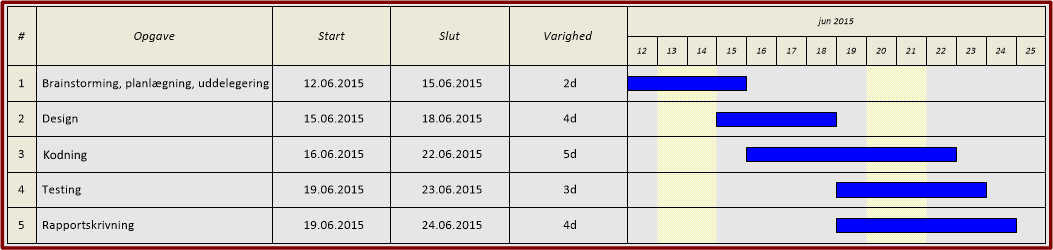
\includegraphics[scale=0.7]{img/Gantt_Chart.png}
\caption{Gantt chart af vores plan}
\end{center}
\end{figure}
 Igennem designfasen blev der kigget på flowcharts, samt skrevet pseudokode. Hen mod slutningen af designfasen blev der skrevet mere og mere reel kode. Kodeskrivningen og testing delen følger hinanden. Sidst i kodefasen blev vi nød til at droppe et af de mål vi havde sat os for at overholde planen, som vi havde lagt og blive færdig med projektet.  De sidste dage op mod deadline blev der skrevet rapport.
\subsection{Problemer}
Under udarbejdelsen af programmet havde vi problemer, som vi ikke havde forudset under design-fasen, vi vil her gennemgå nogle af dem der voldte os mest besvær, at debugge.
\subsubsection{Problemer med realloc}
\label{reallocfejl}
I designfasen havde vi forestillet os at vores boxstruct blot skulle være skrevet som i \textbf{newBoxStack()}, hvor vi dog kun allokerede plads til et enkelt element i hvert array. Ydermere skulle der være en variabel kaldet capacity, der betegnede hvor stort stacket var. Vi ville derefter i \textbf{createBoxes()} undersøge om \textit{*(box).capacity} == \textit{*(box).size} , og hvis det var sandt allokere yderlige 10 pladser med realloc. Dette fungerede dog ikke, og boksene fik tilfældige lokationer på banen. Vi mistænker at der ikke var plads til at dynamisk allokere plads på boardet og finde sammenhængende plads i rammene, og det derfor gik galt. Hvis vi i stedet startede med at allokere plads, gav det os ikke problemer.
\subsubsection{Problemer med knapperne}
Vi havde problemer med knapperne på boardet: Vi var i tvivl om vores kode var dårlig, eller om det var fordi knapperne var slidte og ødelagte. Vi lavede en debouncer, og det hjalp lidt på nogle af knapperne, men vi havde stadig problemer, og nåede aldrig at komme til bunds i problemet. Vi er dog ret overbevist om at problemerne stammer fra de slidte knapper.
\subsection{Test af programmet}
Programmet blev testet op mod vores designkrav og de tekniske specifikationer. Først blev grundelementerne kodet og testet, og når det levede op til specifikationerne blev programmet udvidet med nye funktioner. Koden blev altså skrevet og testet med en buttom up metode, hvor det første element var selve banen. Derefter fulgte strikeren, samt det at kunne få strikeren til at flytte sig. Næste skridt var boldens bevægelse, samt den simple refleksion på kanterne og strikeren, hvor indgangsvinkel var lig udgangsvinkel. Så fulgte kasserne med alle deres egenskaber, og boldens refleksion på kasserne. Endeligt blev strikerens udgangsvinkel ændret alt efter indgangsvinkel. En menu blev lavet sideløbende med spillet. 
Al vores testing blev udført i terminalen, hvor programmet var sat op til at teste, i den forstand, at programmet printede informationer som vi havde  brug for. Dette gjorde vi f.eks. i forbindelse med testing af strikeren, hvor vi printede hvor bolden blev detekteret på strikeren, hvad ind- og udgangsvinklen var. Dette gjorde vi for at checke om vores program opførte sig som forventet.




%\input{tex/Discussion.tex}
%\input{tex/Conclusion.tex}
\section{Dokumentation}

I dette afsnitt er projektets filer, funktioner, moduler og makroer dokumenteret og beskrevet. Fokuset er på funktionernes vigtigste egenskaber og virkemåder. Filerne med tilhørende funktioner er delt op i tre forskellige lag: Application, Application Interface og Hardware Abstraction Layer. Se figur \ref{block}.
 I Application Layer ligger de applikationspecifikke filer, disse filer kan bruges på anden hardware uden at modificere dem. I Hardware Abstraction Layer ligger de hardwarespecifikke filer. Disse filer muligør kommunikation mellem hardware og vores software. Disse filer kan benyttes i helt andre programmer såfremt det er samme type hardware der benyttes. 

\begin{figure}[h]
\begin{center}
\label{block}
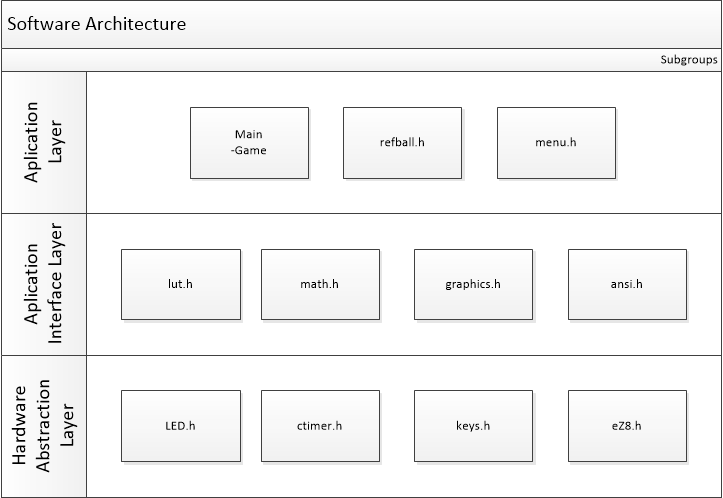
\includegraphics[scale=0.6]{img/SoftwareArchitecture.png}
\caption{Block diagram over de forskellige lag}
\end{center}
\end{figure}
Vi har udviklet alle moduler i fællesskab, og det giver ikke mening at tilskrive nogle personer en særlig del af koden, da meget lidt kode er skrevet af udelukkende en person. 

\subsection{Application layer}
I dette lag findes refball modulet, menu modulet og main modulet.
\subsubsection{main.c}
ReflexBall styres af /textit{main.c} som består af to funktioner. /textbf{main} styrer den overordnede kørsel av programmet og menuen, og /textbf{Game} kontrollerer de forskellige levels og selve gameplayet. Se nærmere beskrivelse af /textbf{main.c} under implementation.

\subsubsection{refball.h}
refball.h er et modul der indeholder grundlæggende regler om spillet: kollision, hvordan bolden skal bevæge sig og hvorledes strikeren skal opføre sig. Desuden indeholder den strukturerne \textit{Ball} og \textit{Box}. Ydermere indeholder dette modul også særligt mange konstanter.
\paragraph{Strukturen Ball}
\textit{Ball} er en stuktur som har variablene opgivet i \ref{Ballkrav}. \textit{outOfBounds}, der fortæller om spilleren er inde for banen, og \textit{powerActivated}, der fortæller om high power er aktiveret, er implementeret som unsigned char's. I \textit{power}, gemmes hvor meget power spilleren har opladet.
 

\paragraph{Strukturen Box}
\textit{Box} er en struktur der indeholder samtlige bokse i spillet. Den indeholder 3 pointere til char-arrays: et koordinatsæt og et tilhørende array med boksenes styrke. Desuden er der to variable der fortæller antallet af bokse der er fyldt i stacket og hvor mange der ikke er ødelagte. I designfasen forestillede vi os at den skulle implementeres som et stack, således arrayernes størrelse var variable, men hvorfor vi ikke gjorde det står i afsnit \ref{reallocfejl}.
\paragraph{void moveBall(Ball * ball)}
Denne funktion flytter bolden ved at tage en peger til en \textit{Ball} som argument og lægger retningsvektoren til x og y koordinaterne.
\paragraph{void moveStriker(long * x,char direction)}
Denne funktion tager to variable som argumenter, en pointer til strikerens x-lokation, og  strikerens retning. Hvis \textit{direction} er 1 bevæger strikeren sig mod positiv x-retning og STRIKER\_SPEED lægges til, ellers bevæger strikeren sig mod negativ x-retning og STRIKER\_SPEED fratrækkes strikerens x-lokation.
\paragraph{unsigned char checkBall(Ball * ball,Box * box,  int x)}\
checkBall() er en funktion som kontrollerer og bestemmer boldens bevægelse. checkBall tager bolden, kasserne og strikerens position som argumenter. I funktionen gennemgåes de forskellige scenarier, hvor bolden kan ramme. Først kontrolleres om strikeren er ramt, derefter om kanterne er ramt og til sidst gennemgås alle kasserne og kontrolleres for om de er ramt. Hvis kassen bliver ramt ændres der i boldens retningsvektor, alt afhængigt af hvordan kassen rammes. Endeligt returnerer funktionen et tegn, svarerende til det, bolden har ramt. Hvis bolden intet har ramt foretages ingen ændring på retningsvektorerne, og et blankt tegn sendes tilbage. 
\paragraph{long toTerminalCoordinates(long x)}\
Denne funktion omdanner tal i 2.14 eller 18.14 til heltal man kan bruge i terminalen. Afrunding laves som vanligvis, ved at afrunde til nærmeste heltal.

\paragraph{void setBallOverStriker( Ball * ball, long st)}
Denne funktion sætter bolden over strikeren.
Funktionen omdanner st til 18.14 format og sætter boldens x-koordinat til dens værdi.
Boldens y-koordinat sættes over strikeren, vha. konstanterne STRIKER\_Y og OVER\_STRIKER, også i 18.14. Boldens retningsvektor sættes derefter til at gå lodret op, og roteres derefter 40 grader mod venstre.
\paragraph{Box * newBoxStack()}
Denne funktion bliver brugt til at lave et nyt \textit{Box}-stack. Der bliver allokeret plads, så der er plads til antallet af bokse givet ved konstanten MAX\_BOXES. Antallet af elementer, \textit{size}, i stacket sættes til 0 og  pegeren til \textit{Box}-stacket.
\paragraph{
void createBoxes( Box * box,char level)}\
Denne funktion tager en peger til Box-stacket og en character der repræsenterer level som argumenter.  Afhængigt af levels værdi, bliver Box-stacket fyldt på en speciel måde, således hvert level er unikt. 

\subsubsection{menu}
Dette modul indeholder funktioner til at tegne og vise grafik når man bevæger sig rundt i menuen.
\paragraph{initiateMenu()}\
Denne funktion renser først skærmen og printer derefter menuen. Slutteligt sættes markøren på Start Game.
\paragraph{moveMarker(int selectedOption)}\
Denne funktion sætter markøren alt afhængigt af inputtet.
\paragraph{void printDifficulty(short diff)}\
Denne funktion har til formål at printe sværhedsgraden når brugeren vælger:
\begin{enumerate}
\item Hvis \textit{diff} er 1, skrives der "Easy"
\item Hvis \textit{diff} er 2, skrives der "Normal"
\item Hvis \textit{diff} er 3, skrives der "Hard"
\end{enumerate}
\paragraph{printHelp()}
Denne funktion printer hjælpe-teksten. Startstedet for teksternes x-koordinat bestemmes af konstanten LEFT\_BORDER

\subsection{Application Interface Layer}
\subsubsection{graphics.h}
Dette modul indeholder grafiske elementer til brug i terminalen. Nogle af funktionerne er særligt udviklet til dette spil, men det er muligt de også ville kunne bruges i andre sammenhæng.  Det kan derfor diskuteres om funktionen strengt taget liger i API-laget. Måske den kan siges at ligge i grænsefeltet.
\paragraph{
void drawBox(unsigned char x, unsigned char y,unsigned char color)}\
Denne funktion tegner en boks med bredden givet ved argumentet og højden 2. Koordinaterne til det øverste venstre hjørne gives som argumenter, sammen med kassens farve, hvor farveskemaet i fgcolor bruges.

\paragraph{void drawChar(unsigned char x, unsigned char y,char tegn)}\
Denne funktion tager et koordinatsæt og et tegn som argumenter. Tegnet bliver skrevet på det givne koordinatsæt.

\paragraph{void moveDrawStriker(unsigned char x, unsigned char direction)}\
heeej

\paragraph{void drawBounds(int x1,int y1, int x2, int y2,unsigned char color)}\
Denne funktion tegner banens kanter. Den tager 2 koordinatsæt som input, x1 og y1 svarende til det øverste venstre hjørne og  x2 og y2 svarende til det nederste højre hjørne. Variablen color bruges til at bestemme farven på kanterne. 

\paragraph{void drawLogo()}\
Denne funktion tegner spillets logo. Den bruger konstanten LEFT\_BORDER til at bestemme på hvilket x-koordinat den skal begynde at skrive fra, således det bliver logoets venstre kant.
drawBall(unsigned char x, unsigned char y, unsigned char color)
Denne funktion tager et koordinatsæt og printer et o i farven bestemt af det 3. parameter.

\paragraph{drawStriker(unsigned char x, unsigned char color, char strikerWidth, char strikerY)}
Denne funktion tegner blot en striker centrummet for strikeren er x, color er farven, strikerWidth er bredden på hver side, og strikerY er Y-koordinatet.

\paragraph{drawGameOver()}
Denne funktion tegner ASCII-kunst af /textit{GAME OVER} og scroller den ud af skærmen.

\paragraph{drawVictory()}
Denne funktion tegner ASCII-kunst af Arnold Schwarzenegger og scroller den ud af skærmen.

\paragraph{scrollText(char y, char delay)}
Denne funktion printer mange linjer med mellemrum sådan at det der tidligere er skrevet bliver scrollet væk.

\paragraph{printExampleBoxes(char x, char y, char boxSize)}
Denne funktion printer de 5 typer bokser der bruges i spillet sådan at brugeren kan se hvor meget de forskellige boksr tåler.

\subsubsection{lut.h}
\label{lut}
Dette modul indeholder en konstant tabel med sinus værdier for en cirkel delt i 512 stykker. Hvis x er vinklen i radian indsættes da blot $\dfrac{x\cdot \pi}{256}$ i tabellen.
\subsubsection{math.h}
Dette modul indeholder nogle generelle matematiske funktioner, heriblandt sin og cosinus, og to makroer til at regne i 2.14 eller 18.14.
\paragraph{Makroer}\
Modulet indeholder to makroer, en til at multiplicere to tal i .14 format, og en til at dividere to tal i .14 format, hhv. FIX14\_MULT(a, b) og FIX14\_div(a,b)

\paragraph{long sin(int x)}\
Denne funktion tager en int som argument. Vinklen skal ikke være i radian, men skal bruge opdelingen af cirklen beskrevet i afsnit \ref{lut}. Der returneres sinus til den givne vinkel.
\paragraph{long cos(int x)}\
Denne funktion tager en int som argument. Vinklen skal ikke være i radian, men skal bruge opdelingen af cirklen beskrevet i afsnit \ref{lut}. Der returneres cosinus til den givne vinkel.
\paragraph{int arcsin(int y)}\
Denne funktion tager en int som argument, og finder arcsinus til integeren. Resultatet returneres med korrekt fortegn, således en negativ int også returnerer en negativ vinkel.
\subsection{Hardware Abstraction Layer}
\subsubsection{keys.h}
Dette modul får inputs fra knapperne, og kan debounce ved hjælp af timer.h
\paragraph{void iniKeys()}
Denne funktion initialiserer den korrekte data-direction på de pins der er forbundne til knapperne, således værdierne kan læses, uden at vi forsøger at skrive outputs samtidigt.

\paragraph{char readKey()}
Denne funktion læser fra knapperne, og returnerer en bit streng, hvor de tre knapper er på hver deres plads i strengen. Hvis pladsen tilhørende knappen er 1, betyder det at knappen bliver trykket. Denne funktion kan godt detektere hvis brugeren trykker flere knapper ind samtidigt. Pladserne er konfigureret således:
\begin{enumerate}
\item Knappen til højre er på LSB(least significant bit)
\item Den midterste knap er på 1. plads i bit-strengen.
\item Knappen til venstre er på 2. plads i bit-strengen.
\end{enumerate}

\paragraph{char getKey}\
Denne funktion bruges hvis man ønsker debouncing. Den læser vha. readKey() og checker derefter om værdien er det samme efter 10 ms og returner dette.
\subsubsection{ctimer.h}
Dette modul har med vores primære timer at gøre. Den har 2 globale variable: \textit{time} og \textit{timeWait}. Time tæller hvor lang tid timeren har været tændt. Grunden til at vi har globable variable her, er fordi timeren skal være uafhængig af main og køre så hurtigt som muligt. Main funktionen kan få adgang til variablene ved nogle setter- og getter-funktioner
\paragraph{void setTimer()}\
Denne funktion sætter vores timer til prescaling 0, continous mode og høj prioritet for interrupt funktionen. Denne timer er sat til at køre hvert ms.
\paragraph{void resetTimer()}\
Denne funktion sætter de til modulet tilhørende globale variable, \textit{time} og \textit{timeWait}, til 0.
\paragraph{void timer0int}\
Dette er interruptfunktionen tilhørende timeren. Den lægger 1 til \textit{time} og trækker 1 fra \textit{timeWait}. 
\paragraph{void SetDelay(int input)}\
Denne funktion sætter timeWait til værdien givet i argumentet. Meningen er at bruge \textit{timeWait} som en slags delay, man kan checke værdien på
\paragraph{getDelay}\
Denne funktion er blot en getter, der returnerer \textit{timeWait}
\paragraph{unsigned long getCentis()}\
Denne funktion er blot en getter, der returnerer \textit{time}
\subsubsection{LED.h}
I dette modul bruges der nogle globale variable. Dette gøres for at f.eks. kunne holde styr på hvilken kolonne og LED-enhet der skal lyse. Det hadde været muligt at undgått brugen af globale variable, men da ville man være nødt til at sende mange flere variable som parametre fra main. Dette ville ikke øge effektiviteten af programmet, men snarere gjort det hele mere kompliceret eftersom dette modul kører på sin egen frekvens. Og siden variablene kun er relevante for modulet er det ikke nogen idé i at de ligger i main.

\paragraph{LEDInit()}
Denne funktion indstiller TIMER1 til at give et interrupt hvert 0.5 ms. Envidere initialiseres de globale variabler i LED.C.

\paragraph{timer1int()}
Denne funktion kaldes af interrupts fra TIMER1 på boardet. Denne funktion kalder funktionen LEDUpdate().

\paragraph{setLedMode(char valueIn)}
Denne funktion er blot en setter der kontrollerer hvilken funktion der kaldes af LEDUpdate.

\paragraph{LEDUpdate()}
Denne funktion kalder en af to funktioner, LEDUpdateOnce() eller LEDUpdatePrint().

\paragraph{LEDSetString(char *string)}
Denne funktion læser en streng  og kopierer den over til den globale variabel /textit{string}. Envidere nulstiller den de globale variable.

\paragraph{LEDLoadBuffer()}
Denne funktion indlæser bufferen fra et karakterset på den måde, at når funktionen LEDUpdatePrint() kaldes er teksten umiddelbart på displayet. Med andre ord; denne funktion gør at teksten ikke ruller ind og er derfor nyttig når man skal opdatere displayet hurtigt.

\paragraph{LEDUpdatePrint()}
Denne funktion bruger tids-multiplexing til at belyse alle kolonnene. For at få dette til at fungere bruges to variable der holder styr på hvilken LED-enhed og kolonne der skal lyse.

\paragraph{LEDUpdateOnce()}
Denne funktion ruller en tekststreng over displayet og holder på de sidste fire tegn. Displayet multiplexes på samme måde som i LEDUpdatePrint(), men strengen bliver også rullet. For at kontrollere hastigheden bruges en tæller.




%\input{tex/Appendix.tex}
\renewcommand{\refname}{\normalfont\selectfont\normalsize Kildeliste} 
\begin{thebibliography}{9}

\bibitem{Yates}
   Randy Yates,
  \emph{Fixed-Point Arithmetic: An Introduction},
   Digital Signal Labs
  23. August
  2007
\bibitem{Dlogic}
	Stephen Brown \& Zvonko Vranesic
	\emph{Fundamentals of Digital Logic with VHDL Design},
	McGraw Hill International Edition , Third Edition,
	2009
\bibitem{Zicomp}
	Zilog,
 \emph{Using the ZiLOG Xtools Z8 Encore! C Compiler},

	http://goo.gl/kUPqL7 , \\ 
	link sidst checket 23-06. Kan ellers findes ved google søgning eller på Zilog's hjemmeside
\bibitem{Zifloat}
	Zilog,
	\emph{Technical Note 
Floating Point Routines} \\
	http://goo.gl/eRBEn0 , \\
	link sidst checket 23-06. Kan ellers findes ved google søgning eller på Zilog's hjemmeside
\end{thebibliography}
\end{document}